\section{Actividad No 03 –  Otros objetos de base de datos} 
		
\begin{enumerate}[1.]
	\item El Departamento de Recursos Humanos requiere ocultar ciertos datos de la tabla EMPLOYEES, Ellos necesitan una vista llamada VW\_Empleados, que contenga los campos ID del Empleado, Nombres e ID del Departamento.
	\item Utilizando la vista anterior crear un reporte que muestre los nombres y departamentos a los cuales
pertenecen los empleados.
	\item El departamento 50 requiere acceso a los datos de los empleados. Generar una vista llamada VW\_Dept50, que contenga las columnas ID del Empleado, Apellidos e ID del Departamento de los empleados del departamento 50. Etiquetar las columnas como EmpNo, Empleado y DeptNo. Por razones de seguridad no se debe permitir a los empleados ser reasignados a otros departamentos.
	\\
	\\CREATE VIEW VW\_Dept50 AS
	\\SELECT employee\_id EmpNo, last\_name employee, department\_id DeptNo
	\\FROM employees
	\\WHERE department\_id = 50;
	\\GO
	\begin{center}
	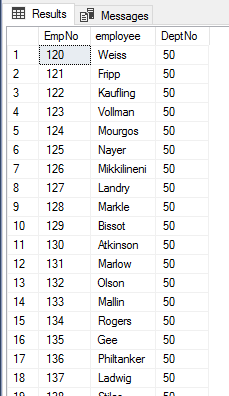
\includegraphics[width=5cm]{./Imagenes/ejercicio3-3} 
	\end{center}
	\item Probar la vista, tratando de reasignar al empleado Matos al departamento 80.
	\\
	\\UPDATE VW\_Dept50
	\\SET DeptNo = 80;
	\\GO
	\begin{center}
	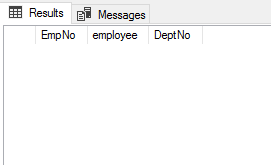
\includegraphics[width=5cm]{./Imagenes/ejercicio3-4} 
	\end{center}

	

	\item Se requiere crear una secuencia que será utilizada en la Llave Primaria de la tabla Departamentos (tabla creada en la práctica anterior). La secuencia deberá iniciar con el valor 200 y terminar en el valor 1000, asimismo deberá incrementarse en 10 cada vez que se requiera. Nombrar la secuencia SEQ\_Departamentos\_ID.
	\\ \\ create sequence SEQ\_Departamentos\_ID start with 200 increment by 10 maxvalue 1000 minvalue 200;	
	
	\begin{center}
	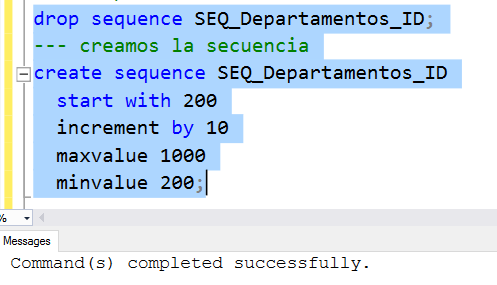
\includegraphics[width=5cm]{./Imagenes/actividad_03_05} 
	\end{center}

	\item Para probar la secuencia, adicionar dos registros a la tabla Departamentos, Educación y Administración. Verificar la adición.
	\\ \\ declare @liCodigo int select @liCodigo = next value for SEQ\_Departamentos\_ID insert into departments  values(@liCodigo,'matematica','300','3300') select * from departments

	\begin{center}
	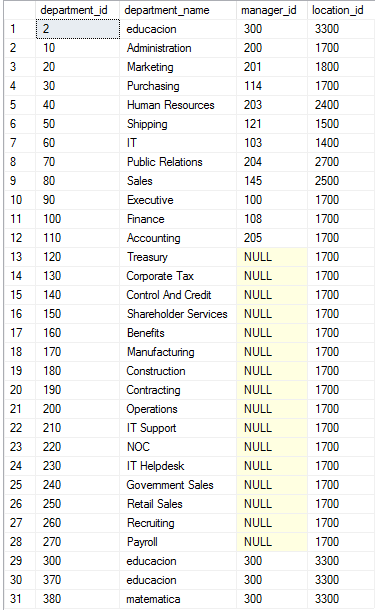
\includegraphics[width=5cm]{./Imagenes/actividad_03_06} 
	\end{center}

	\item Crear un índice no único en la columna NOMBRE de la tabla Departamentos.
	\\ \\CREATE INDEX Indice\_no\_unico ON departments (department\_name);

	\begin{center}
	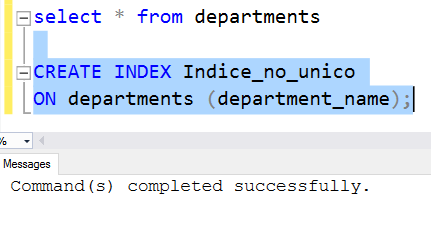
\includegraphics[width=5cm]{./Imagenes/actividad_03_07} 
	\end{center}	

	\item Crear un sinónimo para la tabla EMPLOYEES con el nombre EMP.
	\\ \\EXECUTE sp\_addlinkedserver Server1;  GO CREATE SYNONYM EMP FOR Server1.AdventureWorks2012.HumanResources.Employee; GO 	

	\begin{center}
	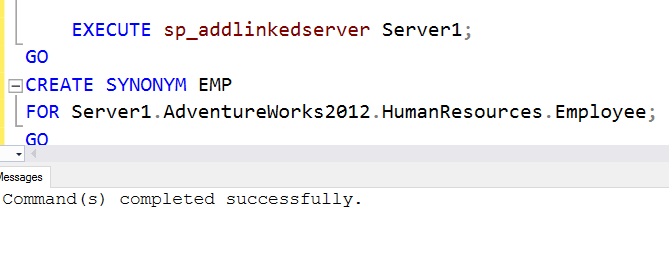
\includegraphics[width=5cm]{./Imagenes/actividad_03_08}  
	\end{center}	

\end{enumerate}

